\documentclass[tikz,border=5pt]{standalone}

\usepackage{tikz}
\usetikzlibrary{arrows.meta}

\begin{document}

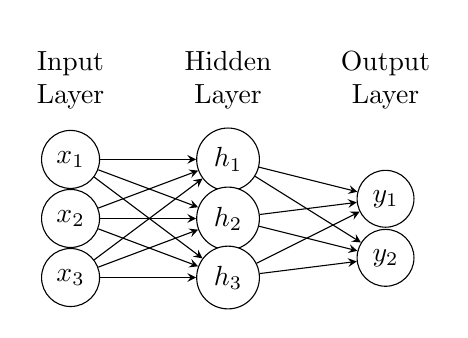
\begin{tikzpicture}[
    neuron/.style={circle, draw=black, fill=white, minimum size=16pt},
    arrow/.style={->, >=stealth}
]
    % Input layer
    \node[neuron] (i1) at (0,1.5) {$x_1$};
    \node[neuron] (i2) at (0,0.75) {$x_2$};
    \node[neuron] (i3) at (0,0) {$x_3$};
    
    % Hidden layer
    \node[neuron] (h1) at (2,1.5) {$h_1$};
    \node[neuron] (h2) at (2,0.75) {$h_2$};
    \node[neuron] (h3) at (2,0) {$h_3$};
    
    % Output layer
    \node[neuron] (o1) at (4,1) {$y_1$};
    \node[neuron] (o2) at (4,0.25) {$y_2$};
    
    % Connections
    \foreach \i in {1,2,3}
        \foreach \j in {1,2,3}
            \draw[arrow] (i\i) -- (h\j);
    
    \foreach \i in {1,2,3}
        \foreach \j in {1,2}
            \draw[arrow] (h\i) -- (o\j);
    
    % Labels
    \node[align=center] at (0,2.6) {\scriptsize \\Input\\Layer};
    \node[align=center] at (2,2.6) {\scriptsize \\Hidden\\Layer};
    \node[align=center] at (4,2.6) {\scriptsize \\Output\\Layer};
\end{tikzpicture}

\end{document}
